\section{Language Sampling}

The sampling method I use is semi-convenience. It is ``semi-'', and not purely convenience, because the languages are chosen randomly from the 100-language sample of WALS. 
I draw a random 20-language list from the 100-language sample, then skim through the reference grammar of the language given in WALS to see if it contains the information I want. 
If the reference grammar is not accessible or it does not provide information on the consonantal distribution for the language, I attempt to find the data in other papers about the language. 
When that also fails, the language is replaced by another language (also chosen randomly from the 100-language sample) from a language family not already presented in the list.

\section{Data Treatment}

\subsection{Phonetics or Phonology?}

In works that consider the representation of phonology and phonetics in great depth like \citet{Boersma1998, Boersma2007}, phonology and phonetics is considered to have at least four levels: Underlying and Surface forms of phonology, and Articulatory and Auditory forms of phonetics.
Phonetic data, in the sense of acoustic signals and articulatory gestures, are probably the most `raw' data that can be used, while phonemes are already subjected to the analysis and perspective of the authors who wrote these grammars. 
Phonemic analysis can produce very different ways of categorizing sounds of a language, which may be justified for the language in question but may not fit for cross-linguistics comparison. 

\begin{figure}[h]
    \centering
    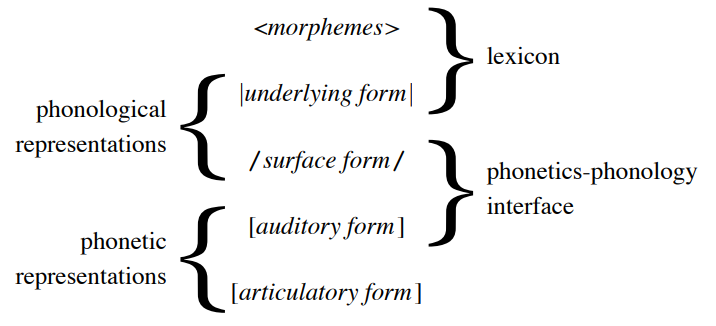
\includegraphics[width=0.75\linewidth]{figures/representation.png}
    \caption{Multi-level representation of phonetics and phonology \citep{Boersma2009}}
    \label{fig:representation}
\end{figure}

Ideally, I should have gathered data at the phonetic levels to have the primary data, but this task is impossible due to two problems.
The first problem is theoretical in that most reference grammars operate on the two levels model of phonetics-phonology: there are the Underlying Form (UF) of phonology, and Surface Form (SF) of phonetics. 
While their Underlying Form may correspond to Underlying Form in Figure \ref{fig:representation}, the degree of phonetic details in their Surface Form is unclear.
The second problem is more practical: most reference grammars do not focus on phonetic details, and so no phonetic data is available to gather from them. 
There are occasionally phonetic remarks, but those are scattered and not made in a systematic manner.

\par
Therefore, I decided to take a practical middle ground and record the data available at the allophonic level. 
For example, if English happens to be on my list then the `clear L' [l] and the `dark L' [ɫ] will be coded as two distinct sounds, with [l] only allowed in the onset, and [ɫ] only in the coda. 

\subsection{Bracket Notation}

The data collected and used in this paper resides, to some extent,between the boundary of phonetic and phonemic, so I have to make certain notation decisions.
In this paper, whenever I refer to the segments that I processed during data collection, I will use the square bracket `[]', since my aim is to record it at phonetic level.
The original reports from reference grammar may vary in terms of phonetic precision, but for the purpose of this paper I will consider them to be equal.
However, when referring to the segments that are used in the argument of other authors, I will respect their use of bracket.

\subsection{Cluster and segmentation}

Consonant clusters will not be considered in this thesis and individual segments in a cluster will be counted separately. However, I will respect the segmentation analysis of the author. Thus, if an author insists that, for instance, [ts] is one segment in this language, it will be coded as a sound distinct from both [t] and [s].

\subsection{Exclusion of certain allophonic variation}

Since the purpose of this thesis is to investigate the distributional asymmetry of consonants relative to the syllable, allophonic variations conditioned by other factors (e.g. as-/dis- similation) will be ignored. 
For example, if in a language, there are [tʃ] and [k] that are in complementary distribution where [tʃ] only appears before front vowels and [k] elsewhere, both of them will be recorded as one segment [k]. 

\par
This decision is not a statement about the real phonological representation of those segments, but merely a way to avoid confounding factors.
An alternative choice is to record both of them separately, but this could disturb the data on positional distribution.
For example, [tʃ] may ends up having higher count and especially in the initial position, because it is quite common to see /t/ and /k/ become [tʃ] in the surface form when followed by /i/ or /j/.
However, in this case the counting of [tʃ] in the initial position is caused partially by the proximity with a sound that has palatal constriction and not purely its position within a syllable.
Arguably, it could also be attributed to the position of the segment (assimilation in the initial position and not in final position), but then we may have to deal with anticipatory versus perseverative assimilation, which is far beyond the scope of this paper. 

\subsection{Data Encoding}

Three positions in the syllable will be distinguishedː initial, medial, and final. Initial and final means onset and coda, and medial means the intervocalic environment. 
If a segment is allowed in a position, it will be coded as 1, otherwise 0. However, if a language prohibits all final consonants, the segments will be coded as ``N/A'' for this position instead.

\par 
In my experience, sometimes the author writes nothing about intervocalic phonotactics. So, following the Maximal Onset Principle (MOP), if the author does not provide any information for the medial position, segments in this position will be assumed to share the same distribution with the initial position. This assumption does not mean that I believe MOP to be true, but it is a practical decision to fill in the gap in the data.

\begin{table}[h!]
    \centering
    \begin{tabular}{| l | l | l | l | l |}
    \hline
     Language & Segment & Initial & Medial & Final \\ \hline
	A & t & 1 & 1 & 1 \\ \hline
	A & d & 1 & 1 & 0 \\ \hline
	... &  &  &  &  \\ \hline
	Z & h & 1 & 0 & N/A \\ \hline
    \end{tabular}
    \caption{Example table}
    \label{tab:example}
\end{table}

\subsection{Data Analysis}

For each segment in each position the number of ``1'' will be divided by the sum of the number of ``1'' and ``0'', yielding a restriction percentage where 1.00 means not restricted while 0.00 means completely not allowed. 


